\documentclass[tikz,border=10pt]{standalone}
\usepackage{tikz}
\usetikzlibrary{shapes.geometric, arrows.meta, positioning, fit, backgrounds, calc}

\definecolor{startend}{RGB}{144,238,144}
\definecolor{process}{RGB}{173,216,230}
\definecolor{decision}{RGB}{255,165,0}
\definecolor{data}{RGB}{255,255,224}
\definecolor{result}{RGB}{230,255,230}
\definecolor{error}{RGB}{255,230,230}
\definecolor{highlight}{RGB}{255,230,204}

\tikzstyle{startstop} = [ellipse, minimum width=3cm, minimum height=1cm, text centered, draw=black, fill=startend, font=\small\bfseries]
\tikzstyle{process} = [rectangle, rounded corners, minimum width=3cm, minimum height=1cm, text centered, draw=black, fill=process, font=\small]
\tikzstyle{decision} = [diamond, aspect=2, minimum width=3cm, minimum height=1cm, text centered, draw=black, fill=decision, font=\small]
\tikzstyle{data} = [rectangle, rounded corners, minimum width=3cm, minimum height=1cm, text centered, draw=black, fill=data, font=\small]
\tikzstyle{action} = [rectangle, rounded corners, minimum width=3cm, minimum height=0.8cm, text centered, draw=black, fill=result, font=\footnotesize]
\tikzstyle{error} = [rectangle, rounded corners, minimum width=3cm, minimum height=0.8cm, text centered, draw=black, fill=error, font=\footnotesize]
\tikzstyle{highlight} = [rectangle, rounded corners, minimum width=3.5cm, minimum height=1.2cm, text centered, draw=black, fill=highlight, font=\small]
\tikzstyle{arrow} = [thick,-{Stealth[length=3mm]}]

\begin{document}
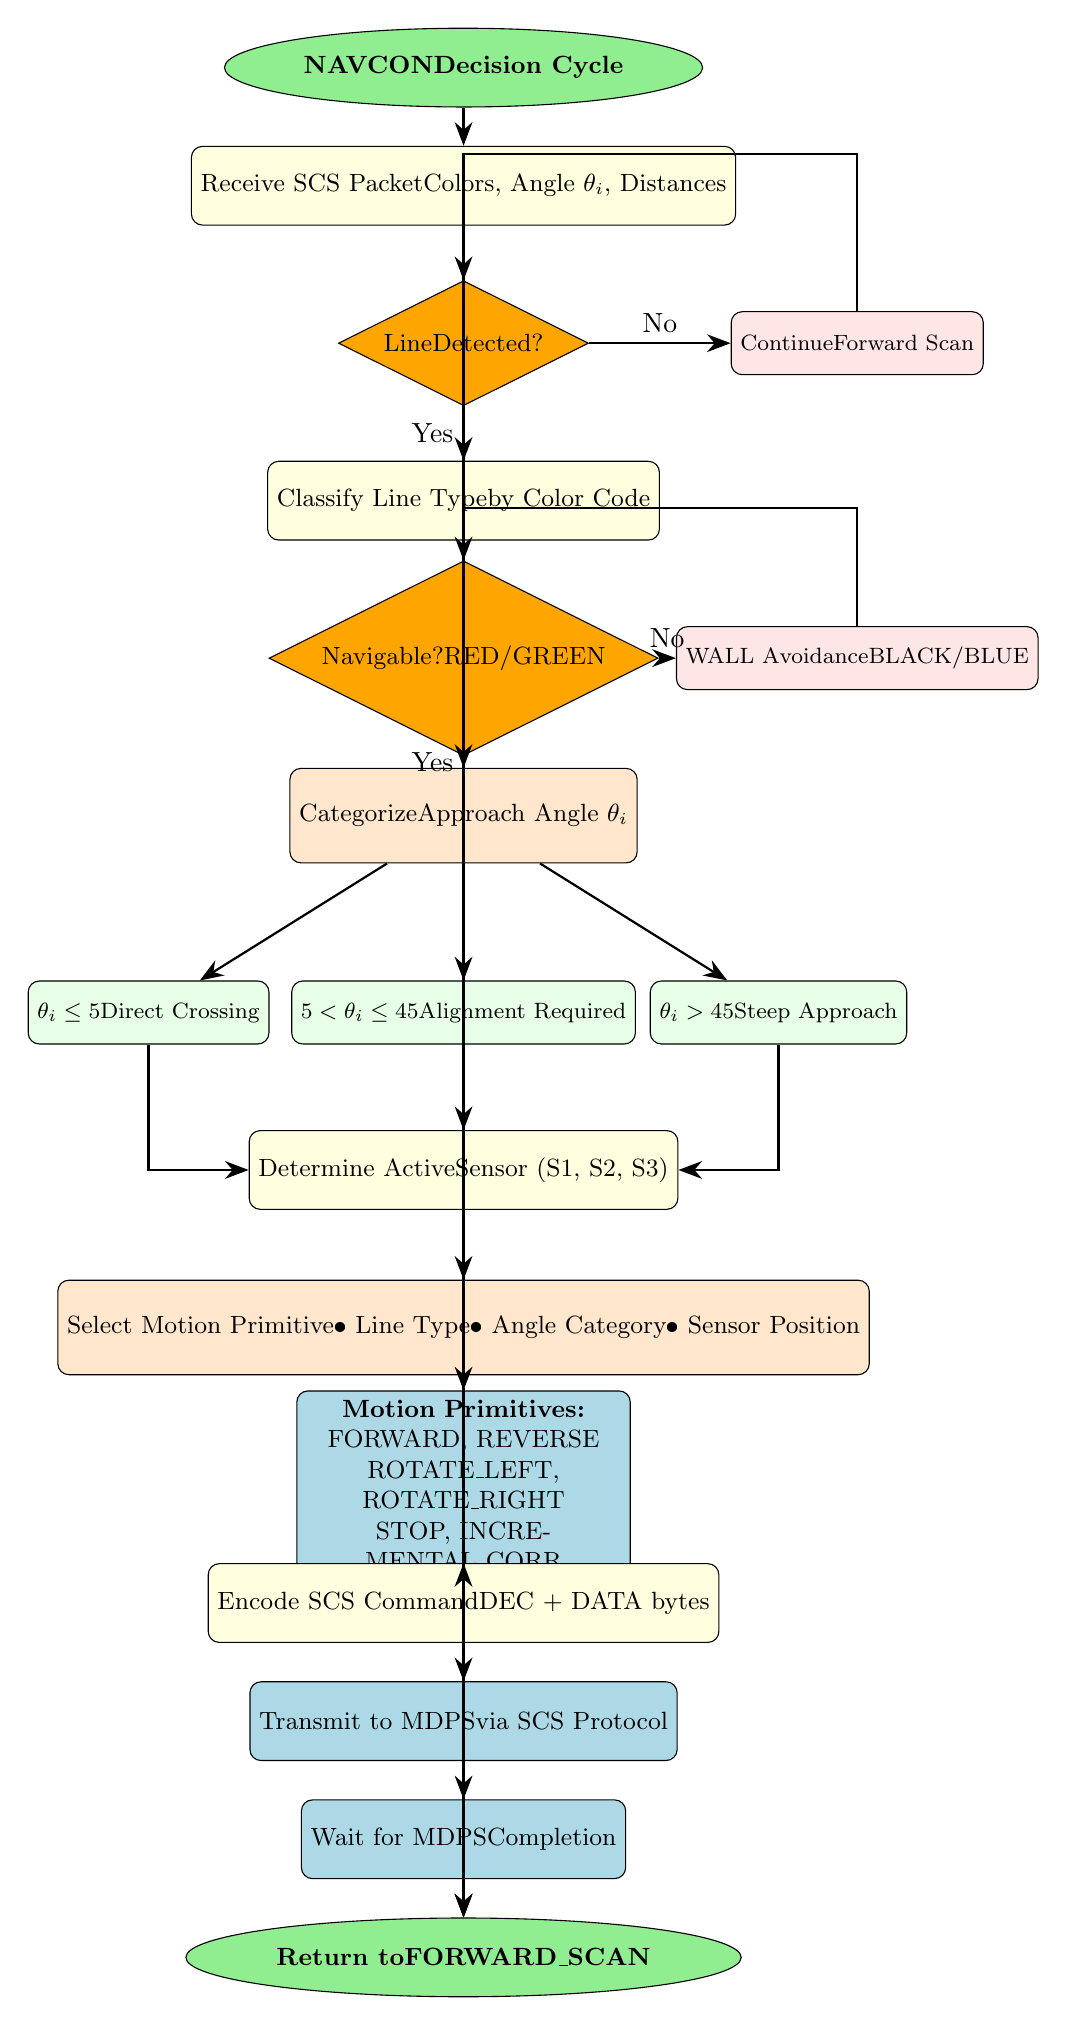
\begin{tikzpicture}[node distance=1.5cm]

% Start
\node (start) [startstop] {NAVCON\\Decision Cycle};

% Input
\node (input) [data, below of=start] {Receive SCS Packet\\Colors, Angle $\theta_i$, Distances};

% Line detection
\node (linecheck) [decision, below of=input, yshift=-0.5cm] {Line\\Detected?};
\node (noline) [error, right of=linecheck, xshift=3.5cm] {Continue\\Forward Scan};

% Line classification
\node (classify) [data, below of=linecheck, yshift=-0.5cm] {Classify Line Type\\by Color Code};
\node (navcheck) [decision, below of=classify, yshift=-0.5cm] {Navigable?\\RED/GREEN};
\node (wall) [error, right of=navcheck, xshift=3.5cm] {WALL Avoidance\\BLACK/BLUE};

% Angle categorization
\node (anglecat) [highlight, below of=navcheck, yshift=-0.5cm] {Categorize\\Approach Angle $\theta_i$};

% Three angle paths
\node (small) [action, below of=anglecat, yshift=-1cm, xshift=-4cm] {$\theta_i \leq 5°$\\Direct Crossing};
\node (medium) [action, below of=anglecat, yshift=-1cm] {$5° < \theta_i \leq 45°$\\Alignment Required};
\node (large) [action, below of=anglecat, yshift=-1cm, xshift=4cm] {$\theta_i > 45°$\\Steep Approach};

% Sensor position
\node (sensor) [data, below of=medium, yshift=-0.5cm] {Determine Active\\Sensor (S1, S2, S3)};

% Motion selection
\node (motion) [highlight, below of=sensor, yshift=-0.5cm] {Select Motion Primitive\\• Line Type\\• Angle Category\\• Sensor Position};

% Primitives list
\node (primitives) [process, below of=motion, yshift=-0.5cm, text width=4cm] {
\textbf{Motion Primitives:}\\
FORWARD, REVERSE\\
ROTATE\_LEFT, ROTATE\_RIGHT\\
STOP, INCREMENTAL\_CORR
};

% Encode
\node (encode) [data, below of=primitives] {Encode SCS Command\\DEC + DATA bytes};

% Transmit
\node (transmit) [process, below of=encode] {Transmit to MDPS\\via SCS Protocol};

% Wait
\node (wait) [process, below of=transmit] {Wait for MDPS\\Completion};

% End
\node (end) [startstop, below of=wait] {Return to\\FORWARD\_SCAN};

% Arrows
\draw [arrow] (start) -- (input);
\draw [arrow] (input) -- (linecheck);
\draw [arrow] (linecheck) -- node[anchor=south] {No} (noline);
\draw [arrow] (linecheck) -- node[anchor=east] {Yes} (classify);
\draw [arrow] (noline) |- ($(noline.north) + (0,2)$) -| (end);

\draw [arrow] (classify) -- (navcheck);
\draw [arrow] (navcheck) -- node[anchor=south] {No} (wall);
\draw [arrow] (navcheck) -- node[anchor=east] {Yes} (anglecat);
\draw [arrow] (wall) |- ($(wall.north) + (0,1.5)$) -| (end);

\draw [arrow] (anglecat) -- (small);
\draw [arrow] (anglecat) -- (medium);
\draw [arrow] (anglecat) -- (large);

\draw [arrow] (small) |- (sensor);
\draw [arrow] (medium) -- (sensor);
\draw [arrow] (large) |- (sensor);

\draw [arrow] (sensor) -- (motion);
\draw [arrow] (motion) -- (primitives);
\draw [arrow] (primitives) -- (encode);
\draw [arrow] (encode) -- (transmit);
\draw [arrow] (transmit) -- (wait);
\draw [arrow] (wait) -- (end);

\end{tikzpicture}
\end{document}
